\documentclass[10pt]{article}
% \usepackage{geometry}
% \geometry{margin=0.2in}
\usepackage[utf8]{inputenc}

\nonstopmode
% \usepackage{minted}[cache=false]
\usepackage{graphicx} % Required for including pictures
\usepackage[figurename=Figure]{caption}
% \usepackage{float}    % For tables and other floats
\usepackage{amsmath}  % For math
\usepackage{amssymb}  % For more math
\usepackage{fullpage} % Set margins and place page numbers at bottom center
% \usepackage{paralist} % paragraph spacing
% \usepackage{subfig}   % For subfigures
%\usepackage{physics}  % for simplified dv, and 
% \usepackage{enumitem} % useful for itemization
% \usepackage{siunitx}  % standardization of si units
\usepackage{hyperref}
% \usepackage{mmacells}
% \usepackage{listings}
% \usepackage{svg}
% \usepackage{xcolor, soul}
\usepackage{bm}
\usepackage{braket}
% \usepackage{cancel}
% \usepackage{setspace}
% \usepackage{listings}
% \usepackage{listings}
% \usepackage[autoload=true]{jlcode}
% \usepackage{pygmentize}

% \definecolor{cambridgeblue}{rgb}{0.64, 0.76, 0.68}

% \sethlcolor{cambridgeblue}

\usepackage[margin=1.8cm]{geometry}
\newcommand{\C}{\mathbb C}
\newcommand{\D}{\bm D}
\newcommand{\R}{\mathbb R}
\newcommand{\Q}{\mathbb Q}
\newcommand{\Z}{\mathbb Z}
\newcommand{\N}{\mathbb N}
\newcommand{\PP}{\mathbb P}
\newcommand{\A}{\mathbb A}
\newcommand{\F}{\mathbb F}
\newcommand{\1}{\mathbf 1}
\newcommand{\ip}[1]{\left< #1 \right>}
\newcommand{\abs}[1]{\left| #1 \right|}
\newcommand{\norm}[1]{\left\| #1 \right\|}

\def\Tr{{\rm Tr}}
\def\tr{{\rm tr}}
\def\Var{{\rm Var}}
\def\calA{{\mathcal A}}
\def\calB{{\mathcal B}}
\def\calD{{\mathcal D}}
\def\calE{{\mathcal E}}
\def\calG{{\mathcal G}}
\def\from{{:}}
\def\lspan{{\rm span}}
\def\lrank{{\rm rank}}
\def\bd{{\rm bd}}
\def\acc{{\rm acc}}
\def\cl{{\rm cl}}
\def\sint{{\rm int}}
\def\ext{{\rm ext}}
\def\lnullity{{\rm nullity}}
% \DeclareSIUnit\clight{\text{\ensuremath{c}}}
% \DeclareSIUnit\fm{\femto\m}
% \DeclareSIUnit\hplanck{\text{\ensuremath{h}}}


% \lstdefinelanguage{julia}%
%   {morekeywords={abstract,break,case,catch,const,continue,do,else,elseif,%
%       end,export,false,for,function,immutable,import,importall,if,in,%
%       macro,module,otherwise,quote,return,switch,true,try,type,typealias,%
%       using,while},%
%    sensitive=true,%
% %    alsoother={$},%
%    morecomment=[l]\#,%
%    morecomment=[n]{\#=}{=\#},%
%    morestring=[s]{"}{"},%
%    morestring=[m]{'}{'},%
% }[keywords,comments,strings]%

% \lstset{%
%     language         = Julia,
%     basicstyle       = \ttfamily,
%     keywordstyle     = \bfseries\color{blue},
%     stringstyle      = \color{magenta},
%     commentstyle     = \color{ForestGreen},
%     showstringspaces = false,
% }

% $
\begin{document}
\begin{center}
	\hrule
	\vspace{.4cm}
	{\textbf { \large CAS PY 452 --- Quantum Physics II}}
\end{center}
Emmy Blumenthal \hspace{\fill} \hspace{\fill}  \textbf{} Discussion Notes\  \\
\textbf{Date:}\  Nov 2, 2022   \hspace{\fill} \textbf{Email:}\ emmyb320@bu.edu \ 
\vspace{.4cm}
\hrule

\section*{WKB approximation for the triangle potential}


\paragraph{Problem:}

Consider the 1D quantum system described by the Hamiltonian,
\begin{align}
	\hat H =
	\frac{\hat p^2}{2m}
	+
	\kappa |\hat x|.
\end{align}
Write the appropriate Bohr-Sommerfeld quantization relation and use the WKB method to approximate the allowed energies of the system.

\paragraph{Solution:}

This is a potential with no `vertical walls', so we use the following quantization rule:
\begin{align}
	\int_{x_1}^{x_2} p(x) dx = \left(n - \frac{1}{2}\right) \pi \hbar,
	\qquad
	n = 1,2,3,\dots
\end{align}
where $p(x)$ satisfies $E = \frac{p(x)^2}{2m}+ \kappa |x|$, and $x_1,x_2$ are the classical turning points (i.e., $p(x_1) = p(x_2) =0$).
Solving, we have,
\begin{gather}
	p(x) = \sqrt{2m(E - \kappa|x|)}\\
	p(x) = 0
	\implies
	E - \kappa|x| = 0 
	\implies
	x_1 = -\frac{E}{\kappa},
	\quad x_2 = + \frac{E}{\kappa}.
\end{gather}
To find the quantization condition, we are left to compute the integral:
\begin{gather}
	\sqrt{2m}
	\int_{-E/\kappa}^{E/\kappa}
	\sqrt{E - \kappa|x|}
	dx
	% &
	=
	2
	\sqrt{2m}
	\int_{0}^{E/\kappa}
	\sqrt{E - \kappa x}
	dx
	=
	2
	\sqrt{2mE^3/\kappa}
	\int_0^{1}
	\sqrt{1 - u} 
	du
	=
	2
	\sqrt{2mE^3/\kappa}
	\int_0^{1}
	\sqrt{v}  
	dv
	\nonumber
	\\
	% &
	=
	\frac{4}{3}\sqrt{2mE^3/\kappa}
	=
	\left(n-\frac{1}{2}\right)\pi\hbar
	\implies
	E_n
	=
	\left(
		\frac{9 \pi^2 \kappa^2\hbar^2}{128 m}
	\right)^{1/3}
	(2n-1)^{2/3}
	,\qquad
	n=1,2,3,\dots.
\end{gather}

\begin{figure}[h!]
	\centering
	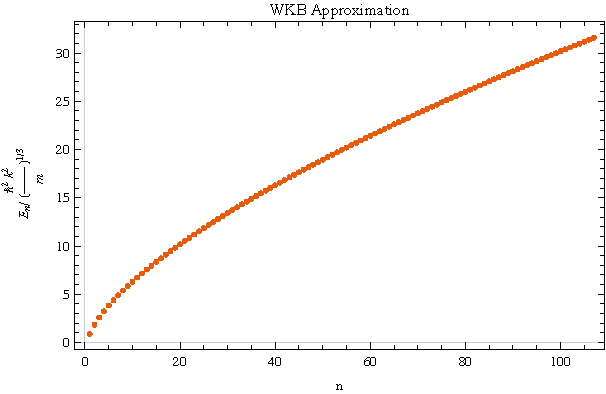
\includegraphics[width=0.7\linewidth]{WKBenergies.pdf}
	\caption{\label{WKBenergies}
		Plot of WKB-approximated energies $E_n$ for various quantum numbers.
	}
\end{figure}

\paragraph{Further notes and comparison with the exact solution:}

If $\left(9 \pi^2 \kappa^2 \hbar^2 / 128m\right)^{1/3} = 0.8853 \times (\kappa^2 \hbar^2 / m)^{1/3}$ is small (i.e. $E^3 \ll \kappa^2 \hbar^2 / m$), then the spacing between energy levels is very small, and the states may seem to form a continuum.
Note that this limit $E^3 \ll \kappa^2 \hbar^2 / m$ is similar to the small $\hbar$ limit.
In this continuum, within a small range $\delta E$, the number of states is $\frac{dn}{dE}\delta E = 
(\frac{d}{dn} E_n)^{-1} \delta E = 
\left(
	\frac{6m}{\pi^2\kappa^2 \hbar^2}
\right)^{1/3} (2n-1)^{1/3}
\delta E
$.
This quantity is the so-called `density of states.'

In the attached {\em Mathematica} notebook, we solve the system exactly for $x>0$ and $x<0$.
Then, we require continuity of the wave-function and its derivative at $x = 0$ in order to obtain a quantization condition for the energies.
In figure \ref{WKBenergies}, the WKB approximate energies are plotted.
In figure \ref{WKBerrors}, the relative errors $|E_\text{WKB} - E_\text{exact}|/|E_\text{exact}|$ are plotted.

\begin{figure}
	\centering
	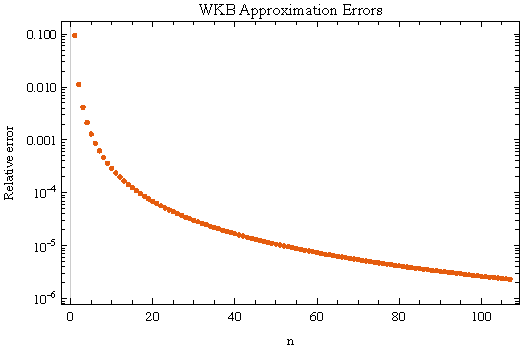
\includegraphics[width=0.7\linewidth]{WKBerrors.pdf}
	\caption{
		\label{WKBerrors}
		Log-scale plot of WKB relative errors.
	}
\end{figure}


\end{document}






